\documentclass[a4paper,11pt]{article}
\usepackage[spanish]{babel}
\usepackage[utf8]{inputenc}

% Configuración páginas
\usepackage{vmargin}							% Márgenes

\usepackage{sectsty}							% Fuente de los títulos
\allsectionsfont{\normalfont \Large \scshape}

\usepackage{graphicx}							% Imágenes
\graphicspath{{images/}}

\usepackage{tabularx}							% Otras tablas
\usepackage{listliketab}						% Tratar indentacion distas como tablas

\usepackage{mathtools}							% Matematicas
\newcommand\numberthis{							% numeración en align*
	\addtocounter{equation}{1}\tag{\theequation}
}

\usepackage{algorithm}							% Algoritmos en latex
\makeatletter
\renewcommand{\ALG@name}{Algoritmo}				% Cambiamos la palabra "Algorithm"
\makeatother
\usepackage{algpseudocode}						% Sintaxis distinta para los algoritmos

% Configuración del título
\newcommand{\horrule}[1]{\rule{\linewidth}{#1}} 	% Horizontal rule

\title{
	\vspace{-25pt}
	\normalfont \Large \textsc{
		Modelos de Investigación Operativa,
        Ingeniería Informática\\
        Universidad de Valladolid
	}\\[10pt]
	\horrule{1pt}\\[10pt]
	\huge \textbf{
		Práctica 10
	}\\
	\horrule{1pt}
}
\author{
	\normalfont \Large Daniel González Alonso
}
\date{
	\normalfont \large \today
}

%%%%%%%%%%%%%%%%%%%%%%%%%%%%%%%%%%%%%%%%%%%%%%%%%%
\begin{document}
\maketitle

%%%% RESUMEN %%%%
\begin{abstract}
	En este documento se describen los problemas y los resultados obtenidos de la práctica 10 del tema 5 de la asignatura Modelos de Investigación Operativa de Ingeniería Informática, Universidad de Valladolid.
\end{abstract}

%%%% DESARROLLO %%%%
\section{Introducción}
Esta práctica trata de problemas TSP (\textit{Travelling Salesman Problem}). Los problemas TSP constan de un grafo ${G=(N,A)}$, donde ${N}$ son los nodos del grafo y ${A}$ los arcos entre éstos, con un coste asociado por cada arco, y el objetivo consiste en encontrar el camino Hamiltoniano (un camino que pase por todos los nodos) de coste mínimo.\\

En esta práctica se nos pide implementar el problema TSP mediante la heurística del entorno más cercano, cuyo esquema es el siguiente:

\begin{algorithm}[!htbp]
\caption{Heurística del entorno más cercano}
\label{alg_entorno_cercano}
\begin{algorithmic}[1]
\State Sea ${j}$ un nodo seleccionado arbitrariamente, ${l=j}$ y ${T=\{1 \ldots n\} - \{l\}}$
\While{$T \neq \emptyset$}
	\State Obtener ${j \in T}$ tal que ${c_{l,j} = \min\left\{ c_{l,i} \mid i \in T \right\}}$
    \State Conectar ${l}$ con ${j}$
    \State ${T \gets T - \{j\}}$
    \State ${l \gets j}$
\EndWhile
\State Conectar ${l}$ con el nodo aleatorio inicial
\end{algorithmic}
\end{algorithm}

%%%%%%%%%%%%%%%%%%%%%%%%%%%%%%%%%%%%%%%%%%%%%%%%%%%%%%
\newpage
\section{Desarrollo}
En esta práctica se nos pide implementar el problema TSP mediante la heurística del entorno más cercano en \textit{Xpress Mosel} y con esta heurística resolver los 5 ejemplos de tamaño ${n = 21}$ puntos con matriz de distancias completa, y los 6 ejemplos Euclídeos de la práctica 9.\\

Estos problemas se encuentran resueltos mediante \textit{Xpress Mosel} en los ficheros \texttt{tsp \ \_entorno\_n21\_1.mos}, \texttt{tsp\_entorno\_n21\_2.mos}, \texttt{tsp\_entorno\_n21\_3.mos}, \texttt{tsp\_entorno\_n21 \ \_4.mos}, \texttt{tsp\_entorno\_n21\_5.mos} en el caso de los ficheros \texttt{n21} y por otro lado para los ficheros \texttt{tsp} Euclídeos en los ficheros \texttt{tsp\_entorno\_tsp\_60\_1.mos}, \texttt{tsp\_entorno\_tsp\_60\_2.mos}, \texttt{tsp\_entorno\_tsp\_60\_3.mos}, \texttt{tsp\_entorno\_tsp\_100\_1.mos}, \texttt{tsp\_entorno\_tsp\_100\_2.mos} y \texttt{tsp\_entorno\_tsp\_100\_3.mos} (el nombre indica el fichero de datos empleado).\\

Antes de explicar la implementación del algoritmo cabe destacar que los costes ${c_{i,j}}$ en nuestro caso son distancias. Para los ficheros \texttt{n21} la matriz de distancias nos viene dada en el mismo fichero. En el caso de los ficheros \texttt{tsp} solo nos vienen las coordenadas de cada nodo, por ello antes de empezar con estos últimos ficheros hay que calcular la matriz de distancias. Para estos fichero la matriz se calculo mediante la distancia Euclídea redondeada al entero más cercano. En caso de la distancia de un nodo a si mismo, se introducía en esta matriz en vez de 0 un valor ``infinito'' (\texttt{MAX\_INT}).\\

La implementación de este algoritmo es muy simple siguiendo el esquema anterior. En mi caso para obtener cualquier ${j}$, a la hora implementar el conjunto ${T}$ simplemente tengo un vector auxiliar llamado \texttt{visitados} de tamaño ${n}$, de forma que cada vez que obtenemos un ${j}$ lo marco en este vector de visitados para que en las siguientes iteraciones no se obtenga el mismo valor de ${j}$. Por otro lado, para las conexiones mantengo un vector llamado \texttt{siguientes}, el cual como indica su nombre, para cada indice almacena el nodo siguiente en el camino de la solución.

\section{Resultados}
Los resultados obtenidos para los ficheros de datos de esta práctica fueron los siguientes:

\begin{table}[!htbp]
\label{results_100}
\centering
\begin{tabularx}{\textwidth}{|p{2cm}|X|X|X|X|X|}
\hline
Problema TSP	& \texttt{n21\_1}	& \texttt{n21\_2}	& \texttt{n21\_3}	& \texttt{n21\_4}	& \texttt{n21\_5} \\ \hline
Distancia Total    & 229    & 219   & 227   & 264   & 220	\\ \hline
Conexiones	& 1 $\to$ 5 $\to$ 21 $\to$ 7 $\to$ 17 $\to$ 4 $\to$ 14 $\to$ 10 $\to$ 18 $\to$ 20 $\to$ 19 $\to$ 11 $\to$ 13 $\to$ 9 $\to$ 12 $\to$ 6 $\to$ 2 $\to$ 16 $\to$ 3 $\to$ 15 $\to$ 8  & 1 $\to$ 4 $\to$ 8 $\to$ 5 $\to$ 9 $\to$ 19 $\to$ 3 $\to$ 15 $\to$ 6 $\to$ 7 $\to$ 20 $\to$ 17 $\to$ 12 $\to$ 16 $\to$ 18 $\to$ 13 $\to$ 21 $\to$ 11 $\to$ 10 $\to$ 2 $\to$ 14  & 1 $\to$ 7 $\to$ 6 $\to$ 20 $\to$ 18 $\to$ 13 $\to$ 12 $\to$ 19 $\to$ 15 $\to$ 16 $\to$ 8 $\to$ 3 $\to$ 5 $\to$ 17 $\to$ 10 $\to$ 9 $\to$ 11 $\to$ 2 $\to$ 21 $\to$ 4 $\to$ 14  & 1 $\to$ 4 $\to$ 13 $\to$ 21 $\to$ 12 $\to$ 5 $\to$ 3 $\to$ 8 $\to$ 10 $\to$ 16 $\to$ 19 $\to$ 18 $\to$ 17 $\to$ 2 $\to$ 6 $\to$ 9 $\to$ 20 $\to$ 11 $\to$ 15 $\to$ 14 $\to$ 7  & 1 $\to$ 8 $\to$ 17 $\to$ 19 $\to$ 21 $\to$ 4 $\to$ 2 $\to$ 9 $\to$ 18 $\to$ 16 $\to$ 10 $\to$ 7 $\to$ 13 $\to$ 11 $\to$ 5 $\to$ 15 $\to$ 6 $\to$ 3 $\to$ 20 $\to$ 14 $\to$ 12	\\ \hline
\end{tabularx}
\caption{Comparación de los resultados de los ficheros \texttt{n21}}
\end{table}


\begin{table}[!htbp]
\label{results_tsp_60}
\centering
\begin{tabularx}{\textwidth}{|p{2cm}|X|X|X|}
\hline
Problema TSP    & \texttt{tsp\_60\_1}   & \texttt{tsp\_60\_2}   & \texttt{tsp\_60\_3}	\\ \hline
Distancia Total & 786   & 784   & 779	\\ \hline
Conexiones	& 1 $\to$ 35 $\to$ 53 $\to$ 27 $\to$ 23 $\to$ 47 $\to$ 55 $\to$ 28 $\to$ 16 $\to$ 34 $\to$ 4 $\to$ 29 $\to$ 25 $\to$ 19 $\to$ 9 $\to$ 43 $\to$ 56 $\to$ 18 $\to$ 37 $\to$ 14 $\to$ 24 $\to$ 52 $\to$ 45 $\to$ 3 $\to$ 33 $\to$ 2 $\to$ 7 $\to$ 17 $\to$ 38 $\to$ 41 $\to$ 60 $\to$ 49 $\to$ 40 $\to$ 21 $\to$ 36 $\to$ 11 $\to$ 44 $\to$ 59 $\to$ 5 $\to$ 42 $\to$ 48 $\to$ 32 $\to$ 8 $\to$ 12 $\to$ 20 $\to$ 51 $\to$ 54 $\to$ 39 $\to$ 31 $\to$ 50 $\to$ 58 $\to$ 15 $\to$ 26 $\to$ 6 $\to$ 57 $\to$ 46 $\to$ 30 $\to$ 13 $\to$ 22 $\to$ 10	& 1 $\to$ 57 $\to$ 58 $\to$ 49 $\to$ 59 $\to$ 41 $\to$ 31 $\to$ 23 $\to$ 48 $\to$ 42 $\to$ 36 $\to$ 53 $\to$ 20 $\to$ 2 $\to$ 17 $\to$ 3 $\to$ 38 $\to$ 55 $\to$ 6 $\to$ 33 $\to$ 45 $\to$ 21 $\to$ 16 $\to$ 43 $\to$ 8 $\to$ 40 $\to$ 50 $\to$ 56 $\to$ 15 $\to$ 37 $\to$ 24 $\to$ 32 $\to$ 12 $\to$ 35 $\to$ 11 $\to$ 22 $\to$ 52 $\to$ 46 $\to$ 51 $\to$ 18 $\to$ 27 $\to$ 5 $\to$ 13 $\to$ 29 $\to$ 4 $\to$ 44 $\to$ 7 $\to$ 54 $\to$ 34 $\to$ 26 $\to$ 60 $\to$ 10 $\to$ 14 $\to$ 47 $\to$ 39 $\to$ 19 $\to$ 25 $\to$ 9 $\to$ 28 $\to$ 30	& 1 $\to$ 9 $\to$ 4 $\to$ 38 $\to$ 49 $\to$ 40 $\to$ 32 $\to$ 13 $\to$ 35 $\to$ 36 $\to$ 8 $\to$ 37 $\to$ 59 $\to$ 52 $\to$ 18 $\to$ 23 $\to$ 56 $\to$ 48 $\to$ 58 $\to$ 14 $\to$ 16 $\to$ 44 $\to$ 45 $\to$ 42 $\to$ 17 $\to$ 47 $\to$ 55 $\to$ 3 $\to$ 19 $\to$ 51 $\to$ 5 $\to$ 21 $\to$ 11 $\to$ 7 $\to$ 30 $\to$ 25 $\to$ 31 $\to$ 57 $\to$ 34 $\to$ 2 $\to$ 10 $\to$ 15 $\to$ 54 $\to$ 60 $\to$ 41 $\to$ 6 $\to$ 28 $\to$ 12 $\to$ 22 $\to$ 20 $\to$ 29 $\to$ 43 $\to$ 39 $\to$ 53 $\to$ 46 $\to$ 33 $\to$ 26 $\to$ 24 $\to$ 50 $\to$ 27	\\ \hline
\end{tabularx}
\caption{Comparación de los resultados de los ficheros \texttt{tsp\_60}}
\end{table}

\begin{table}[!htbp]
\label{results_tsp_100}
\centering
\begin{tabularx}{\textwidth}{|p{2cm}|X|X|X|}
\hline
Problema TSP    & \texttt{tsp\_100\_1}  & \texttt{tsp\_100\_2}  & \texttt{tsp\_100\_3}  \\ \hline
Distancia Total & 1005   & 973   & 965	\\ \hline
Conexiones	& 1 $\to$ 24 $\to$ 41 $\to$ 59 $\to$ 57 $\to$ 40 $\to$ 31 $\to$ 64 $\to$ 80 $\to$ 63 $\to$ 36 $\to$ 47 $\to$ 99 $\to$ 4 $\to$ 67 $\to$ 79 $\to$ 82 $\to$ 19 $\to$ 45 $\to$ 97 $\to$ 39 $\to$ 81 $\to$ 33 $\to$ 100 $\to$ 3 $\to$ 73 $\to$ 75 $\to$ 28 $\to$ 86 $\to$ 27 $\to$ 29 $\to$ 92 $\to$ 78 $\to$ 5 $\to$ 69 $\to$ 20 $\to$ 43 $\to$ 76 $\to$ 49 $\to$ 95 $\to$ 13 $\to$ 48 $\to$ 11 $\to$ 12 $\to$ 42 $\to$ 16 $\to$ 61 $\to$ 26 $\to$ 84 $\to$ 14 $\to$ 83 $\to$ 37 $\to$ 77 $\to$ 60 $\to$ 38 $\to$ 88 $\to$ 96 $\to$ 85 $\to$ 70 $\to$ 94 $\to$ 44 $\to$ 89 $\to$ 21 $\to$ 87 $\to$ 91 $\to$ 34 $\to$ 7 $\to$ 22 $\to$ 90 $\to$ 62 $\to$ 58 $\to$ 46 $\to$ 35 $\to$ 54 $\to$ 68 $\to$ 98 $\to$ 8 $\to$ 93 $\to$ 50 $\to$ 2 $\to$ 66 $\to$ 52 $\to$ 32 $\to$ 53 $\to$ 72 $\to$ 17 $\to$ 25 $\to$ 10 $\to$ 23 $\to$ 71 $\to$ 65 $\to$ 18 $\to$ 74 $\to$ 6 $\to$ 15 $\to$ 9 $\to$ 55 $\to$ 56 $\to$ 30 $\to$ 51	& 1 $\to$ 87 $\to$ 20 $\to$ 31 $\to$ 16 $\to$ 23 $\to$ 76 $\to$ 63 $\to$ 98 $\to$ 78 $\to$ 77 $\to$ 86 $\to$ 9 $\to$ 55 $\to$ 53 $\to$ 51 $\to$ 26 $\to$ 6 $\to$ 59 $\to$ 57 $\to$ 8 $\to$ 5 $\to$ 82 $\to$ 45 $\to$ 22 $\to$ 65 $\to$ 14 $\to$ 4 $\to$ 35 $\to$ 92 $\to$ 62 $\to$ 11 $\to$ 24 $\to$ 84 $\to$ 39 $\to$ 54 $\to$ 67 $\to$ 27 $\to$ 75 $\to$ 47 $\to$ 37 $\to$ 42 $\to$ 68 $\to$ 94 $\to$ 48 $\to$ 44 $\to$ 71 $\to$ 34 $\to$ 56 $\to$ 81 $\to$ 13 $\to$ 21 $\to$ 12 $\to$ 99 $\to$ 38 $\to$ 66 $\to$ 73 $\to$ 19 $\to$ 43 $\to$ 74 $\to$ 40 $\to$ 7 $\to$ 64 $\to$ 83 $\to$ 41 $\to$ 60 $\to$ 15 $\to$ 90 $\to$ 36 $\to$ 30 $\to$ 17 $\to$ 10 $\to$ 58 $\to$ 29 $\to$ 72 $\to$ 18 $\to$ 33 $\to$ 70 $\to$ 88 $\to$ 91 $\to$ 100 $\to$ 69 $\to$ 95 $\to$ 2 $\to$ 49 $\to$ 46 $\to$ 25 $\to$ 61 $\to$ 85 $\to$ 32 $\to$ 3 $\to$ 50 $\to$ 93 $\to$ 80 $\to$ 79 $\to$ 97 $\to$ 89 $\to$ 52 $\to$ 96 $\to$ 28	& 1 $\to$ 16 $\to$ 60 $\to$ 22 $\to$ 46 $\to$ 71 $\to$ 95 $\to$ 88 $\to$ 67 $\to$ 68 $\to$ 27 $\to$ 90 $\to$ 30 $\to$ 25 $\to$ 21 $\to$ 97 $\to$ 73 $\to$ 34 $\to$ 63 $\to$ 92 $\to$ 14 $\to$ 96 $\to$ 3 $\to$ 45 $\to$ 78 $\to$ 28 $\to$ 82 $\to$ 56 $\to$ 52 $\to$ 54 $\to$ 13 $\to$ 48 $\to$ 40 $\to$ 81 $\to$ 7 $\to$ 62 $\to$ 70 $\to$ 17 $\to$ 6 $\to$ 64 $\to$ 77 $\to$ 15 $\to$ 26 $\to$ 61 $\to$ 35 $\to$ 37 $\to$ 83 $\to$ 39 $\to$ 80 $\to$ 58 $\to$ 51 $\to$ 76 $\to$ 91 $\to$ 74 $\to$ 65 $\to$ 29 $\to$ 38 $\to$ 44 $\to$ 79 $\to$ 36 $\to$ 33 $\to$ 89 $\to$ 84 $\to$ 41 $\to$ 75 $\to$ 47 $\to$ 24 $\to$ 20 $\to$ 4 $\to$ 42 $\to$ 55 $\to$ 18 $\to$ 57 $\to$ 99 $\to$ 66 $\to$ 94 $\to$ 10 $\to$ 12 $\to$ 86 $\to$ 85 $\to$ 11 $\to$ 53 $\to$ 32 $\to$ 5 $\to$ 50 $\to$ 8 $\to$ 9 $\to$ 59 $\to$ 87 $\to$ 43 $\to$ 31 $\to$ 72 $\to$ 2 $\to$ 23 $\to$ 98 $\to$ 69 $\to$ 19 $\to$ 100 $\to$ 93 $\to$ 49	\\ \hline
\end{tabularx}
\caption{Comparación de los resultados de los ficheros \texttt{tsp\_100}}
\end{table}

\clearpage
También obtuve los gráficos IVE para los ficheros \texttt{tsp}. En este caso aquí se muestra el resultado obtenido para el fichero \texttt{tsp\_100\_1}:

\begin{figure}[!htbp]
	\centering
	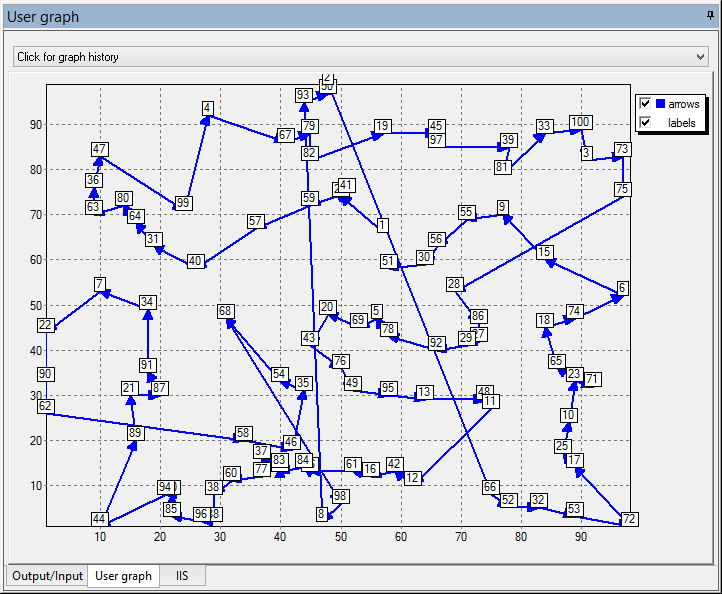
\includegraphics[width=1.0\textwidth]{entorno_100_1.png}
\end{figure}

\end{document}
